\noindent

\includegraphics[height=1.25cm]{images/pictograms/benchmark}

\includegraphics[height=1.25cm]{images/pictograms/under_construction}

\includegraphics[height=1.25cm]{images/pictograms/FEM}

\includegraphics[height=1.25cm]{images/pictograms/paraview}


%%%%%%%%%%%%%%%%%%%%%%%%%%%%%%%%%%%%%%%%%%%%%%%%%%%%%%%%%%%%%%%%%%%%%%%%%%%%%%%%%%%%%%%%%%%%%%%%%%%

\begin{flushright} {\tiny {\color{gray} python\_codes/fieldstone\_147/text.tex}} \end{flushright}

%\lstinputlisting[language=bash,basicstyle=\small]{python_codes/template_keywords.key}

\par\noindent\rule{\textwidth}{0.4pt}

\begin{center}
\inpython
{\small Code: \url{https://github.com/cedrict/fieldstone/tree/master/python_codes/fieldstone_147}}
\end{center}

\par\noindent\rule{\textwidth}{0.4pt}

%%%%%%%%%%%%%%%%%%%%%%%%%%%%%%%%%%%%%%%%%%%%%%%%%%%%%%%%%%%%%%%%%%%%%%%%%%%%%%%%%%%%%%%%%%%%%%%%%%%

The idea behind this \stone is the comparison of various approaches to solve the 
Stokes system.
We have three methods:
\begin{itemize}
\item build the system as a single (sparse) two-dimensional array and use 
spsolve\footnote{\url{https://docs.scipy.org/doc/scipy/reference/generated/scipy.sparse.linalg.spsolve.html}}. It looks like it is the SuperLU solver\footnote{\url{https://caam37830.github.io/book/02_linear_algebra/sparse_linalg.html}} 
\item use UMFPACK option of spsolve
\item build the system as a single (sparse) two-dimensional array and use (l)gmres;
\item build the $\K$ and $\G$ blocks and use conjugate gradient method on 
the Schur complement equation ('SC-CG'), as explained in Section~\ref{MMM-ss:schurpcg}.
This solver is is {\tt schur\_complement\_cg\_solver.py}
\end{itemize}
All three methods should also be used with a preconditioner.

This \stone is \stone~\ref{f18}.

%==================================
\section*{Without preconditioner}

\begin{center}
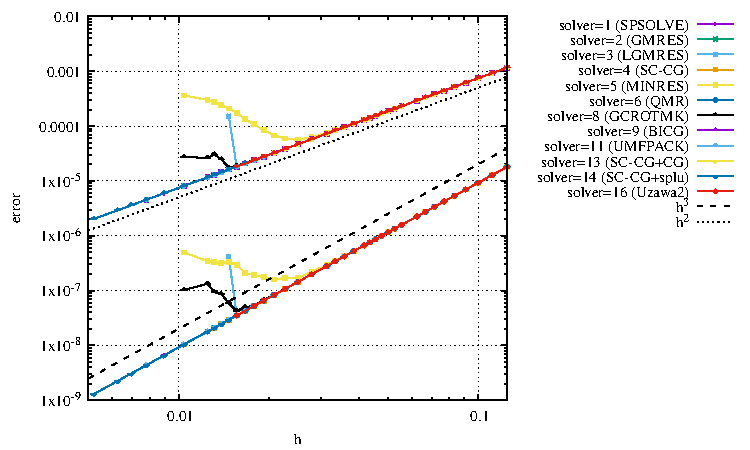
\includegraphics[width=12cm]{python_codes/fieldstone_147/RESULTS/errors.pdf}
\end{center}

\begin{center}
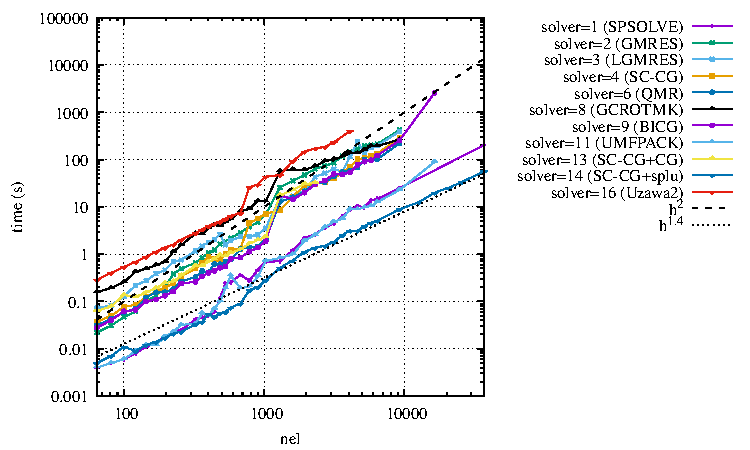
\includegraphics[width=12cm]{python_codes/fieldstone_147/RESULTS/solve.pdf}\\
{\captionfont Time to solve linear system. Only results for usable solvers are shown.}
\end{center}

\begin{center}
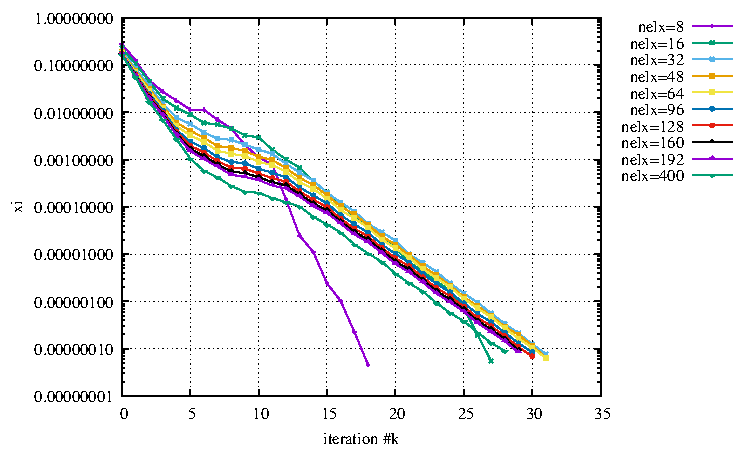
\includegraphics[width=12cm]{python_codes/fieldstone_147/RESULTS/convergence_schur_cpl.pdf}\\
{\captionfont Convergence of the SC-CG solver as function of resolution.}
\end{center}

\begin{center}
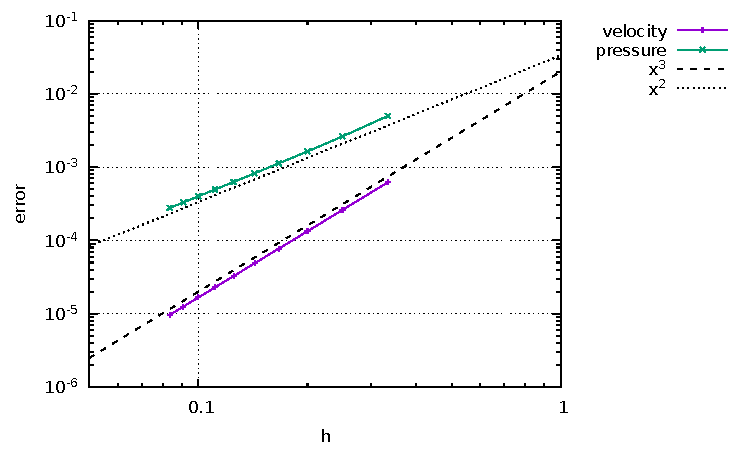
\includegraphics[width=12cm]{python_codes/fieldstone_147/RESULTS/tol_study_solver4/errors.pdf}\\
{\captionfont Influence of the relative tolerance on the accuracy of the solution obtained 
with the SC-CG solver.}
\end{center}

Conclusions:

\begin{itemize}
\item my own Schur complement CG solver rivals other LINALG solvers 
\item MINRES, even with very low tolerance, ultimately fails
\item TFQMR simply no
\item BICGSTAB simply no
\item GCROTMK usable but slowest, also crashes sometimes
\end{itemize}



%%%%%%%%%%%%%%%%%%%%%%%%%%%%%%%%%%%%%%%%%%%%%%%%%%%%%%%%%%%%%%%%%%%%%%%%%%%%%%%%%%%%%%%%%%%%%%%%%%%
\par\noindent\rule{\textwidth}{0.4pt}

\vspace{.5cm}

\begin{center}
\fbox{\begin{minipage}{0.9\textwidth}
{\color{teal}To Do, open questions, future work?}
\begin{itemize}
\item do smthg
\end{itemize}
\end{minipage}}
\end{center}

%%%%%%%%%%%%%%%%%%%%%%%%%%%%%%%%%%%%%%%%%%%%%%%%%%%%%%%%%%%%%%%%%%%%%%%%%%%%%%%%%%%%%%%%%%%%%%%%%%%
\vspace{.5cm}

\Literature:\\
\fullcite{xxxxYY}







